\documentclass[12pt]{article}

% --- Encoding ---
\usepackage[T1]{fontenc}

% --- Core packages ---
\usepackage[margin=1in]{geometry}
\usepackage{amsmath}
\usepackage{amssymb}
\usepackage{graphicx}
\usepackage{booktabs}
\usepackage{array}
\usepackage{enumitem}
\usepackage{titlesec}
\usepackage{abstract}
\usepackage{setspace}

% --- Citation style: natbib with sort+compress ---
\usepackage[numbers,sort&compress]{natbib}

% --- TikZ ---
\usepackage{tikz}
\usetikzlibrary{shapes.geometric, arrows.meta, positioning, fit, backgrounds, shadows}
\usepackage{xcolor}

% --- Headers and footers ---
\usepackage{fancyhdr}

% --- Hyperref last ---
\usepackage{hyperref}

% --- Colors ---
\definecolor{humanblue}{RGB}{30, 90, 160}
\definecolor{aigreen}{RGB}{40, 140, 80}
\definecolor{detgray}{RGB}{90, 90, 110}
\definecolor{lightgray}{RGB}{245, 245, 248}
\definecolor{warnorange}{RGB}{200, 100, 20}

% --- Custom semantic commands for consistency ---
\newcommand{\bxthree}{\textbf{BX3}}
\newcommand{\purpose}{\textit{Purpose Layer}}
\newcommand{\bounds}{\textit{Bounds Engine}}
\newcommand{\fact}{\textit{Fact Layer}}

% --- Header/Footer ---
\pagestyle{fancy}
\fancyhf{}
\rhead{\small Beebe — Bxthre3 Inc}
\lhead{\small The BX3 Framework v1.0}
\cfoot{\thepage}
\renewcommand{\headrulewidth}{0.4pt}

% --- Hyperref metadata ---
\hypersetup{
    colorlinks=true,
    linkcolor=humanblue,
    citecolor=humanblue,
    urlcolor=humanblue,
    pdftitle={The BX3 Framework: A Universal Architecture of Functional Roles for Purpose, Bounded Reasoning, and Deterministic Fact},
    pdfauthor={Jeremy Blaine Thompson Beebe},
    pdfsubject={Artificial Intelligence, Software Architecture, AI Governance},
    pdfkeywords={BX3 Framework, Purpose Layer, Bounds Engine, Fact Layer, artificial intelligence, deterministic systems, software architecture, human-in-the-loop, upstream accountability, autonomous systems, AI governance, sociotechnical systems, edge computing},
    pdfcreator={pdfLaTeX},
    bookmarksnumbered=true,
    breaklinks=true,
}

\title{
    \vspace{1.2cm}
    {\LARGE \textbf{The BX3 Framework:}}\\[0.6em]
    {\large \textit{Implementation Protocols for Accountable Autonomous Systems}}\\[1.0em]
    {\normalsize Three Functional Layers. Five Named Protocols. Guaranteed Upstream Accountability.}
}

\author{
    \textbf{Jeremy Blaine Thompson Beebe}\\[0.2em]
    \textit{Independent Researcher}\\[0.3em]
    \textit{Preprint — Bxthre3 Inc, April 2026}\\[0.3em]
}

\date{April 2026}

\begin{document}

\maketitle
\thispagestyle{fancy}

\begin{abstract}
\noindent
The current discourse around artificial intelligence frequently presents a false binary: either AI will replace traditional software systems, or it is merely a productivity tool of limited consequence. This paper argues that both positions miss a more fundamental and practically useful insight. We propose the \textbf{BX3 Framework} --- a universal architectural model organized around three immutable functional layers: the \textit{Purpose Layer}, which provides intent, judgment, and accountability; the \textit{Bounds Engine}, which provides interpretation, bounded reasoning, and constrained execution; and the \textit{Fact Layer}, which provides deterministic enforcement, hard physical constraint, and forensic auditability.

Critically, the BX3 Framework does not prescribe \textit{who} or \textit{what} occupies each layer. It prescribes the \textit{functional properties} each layer must maintain --- and holds any actor occupying that layer to those properties regardless of their nature. A human, an AI system, or a mechanical process may each legitimately occupy any layer, provided they satisfy that layer's functional requirements. This actor-agnostic, function-centered definition makes the framework universally applicable across human organizations, fully automated systems, multi-agent AI architectures, and any hybrid composition.

A core safety property of the framework is its upstream accountability guarantee: when any node encounters a state it cannot resolve within its bounds, accountability escalates recursively upward through the system hierarchy --- bypassing all machine actors --- until it reaches a human anchor. \textit{The system fails upward into human consciousness --- never downward into algorithmic chaos.}

We demonstrate that when these three functional layers are clearly separated and their properties enforced by design, systems become simultaneously more capable and less complex. We further argue that the Bounds Engine is most powerfully employed not as a replacement for the Fact Layer but as a tool for designing, accelerating, and improving it. We show that the BX3 Framework is not merely a software engineering principle but a universal structural pattern observable across law, medicine, autonomous systems, organizational design, and biological cognition. A companion engineering specification --- the BX3 Protocol --- is in preparation and will provide normative, certifiable implementation standards derived from this framework.

\vspace{0.5em}
\noindent\textit{This paper is a conceptual framework and position paper. Empirical validation studies are currently in development by the author and will be published as subsequent work. This preprint establishes the theoretical foundation and research agenda that those studies will address.}
\end{abstract}

\vspace{0.5em}
\noindent\textbf{Keywords:} BX3 Framework, Purpose Layer, Bounds Engine, Fact Layer, artificial intelligence, deterministic systems, software architecture, human-in-the-loop, upstream accountability, recursive systems, autonomous systems, AI governance, sociotechnical systems, agentic systems, edge computing

\vspace{1em}
\hrule
\vspace{1em}

\onehalfspacing

% -------------------------------------------------------
\section{Introduction}
\label{sec:intro}

The rapid advancement and deployment of large language models and AI-based systems has generated significant confusion about the appropriate role of AI within engineered systems. A prevalent narrative suggests that AI will progressively replace traditional deterministic software, eventually subsuming most computational tasks. A counter-narrative dismisses AI as a novelty, inadequate for the reliability demands of production systems.

Both narratives fail engineers, architects, and decision-makers in the same fundamental way: they offer no principled model for how these technologies relate to one another or how they should be combined in practice. The result is systems that are either over-reliant on AI where determinism is required, or unnecessarily constrained by legacy deterministic thinking where AI could genuinely help.

This paper proposes a clarifying framework: the \textbf{BX3 Framework}. The framework organizes any complex system into three immutable functional layers --- the \textit{Purpose Layer}, the \textit{Bounds Engine}, and the \textit{Fact Layer} --- each defined by the properties it must maintain rather than by the type of actor that occupies it.

This actor-agnostic, function-centered definition is the framework's most important architectural property. A human, an AI system, or a mechanical process may each legitimately occupy any layer of the BX3 Framework --- provided they satisfy the functional requirements of that role. What the framework prescribes is not \textit{who} belongs in each layer but \textit{what properties} each layer must maintain for the system as a whole to be reliable, governable, and certifiable.

A companion engineering specification --- the BX3 Protocol --- is in preparation and will provide normative, certifiable implementation standards derived from this theoretical foundation.

We further argue that the BX3 Framework is not a novel invention but a synthesis of well-established principles --- separation of concerns \cite{dijkstra1982}, sociotechnical systems theory \cite{trist1981}, control theory \cite{wiener1948}, and human-in-the-loop design \cite{bansal2019} --- applied to the specific and urgent challenge of AI integration in the current technological moment. Its value lies not in the novelty of its components but in the clarity, universality, and completeness of their unification.

\textit{Note: The first-person plural ``we'' is used throughout in the conventional academic sense, consistent with single-author scholarly writing.}

% -------------------------------------------------------
\section{Defining the Three Functional Layers}
\label{sec:layers}

The BX3 Framework defines three functional layers. Each layer is defined by the \textit{properties it must maintain}, not by the type of actor that occupies it. A human, an AI system, a mechanical process, an institution, or any combination thereof may occupy any layer --- provided the functional requirements of that layer are satisfied.

This actor-agnostic definition is deliberate and essential. It makes the framework applicable to human-only organizations, to fully automated systems, to multi-agent AI architectures, and to any hybrid composition. It also resolves the false question of whether AI will ``replace'' humans in any given role: the question is not who occupies the layer, but whether the occupant satisfies the layer's functional requirements.

\subsection{Layer 1: The Purpose Layer}

The Purpose Layer is responsible for \textit{intent}, \textit{judgment}, and \textit{accountability}. It sets Service Level Objectives, strategic goals, and the ``why'' that governs all downstream activity. Whatever occupies this layer must be capable of:

\begin{itemize}[noitemsep]
    \item Defining the goals the system exists to achieve and why.
    \item Making trade-off decisions under genuine uncertainty, where no algorithmic optimum exists.
    \item Holding accountability for outcomes --- answering for the system's behavior to external parties.
    \item Asking and answering ``why are we building this, and for whom?''
    \item Updating goals when context changes in ways the system was not designed to anticipate.
\end{itemize}

In the current technological moment, the Purpose Layer must remain anchored to a \textit{human accountability anchor} --- an individual or institution capable of bearing legal and ethical responsibility for the system's actions. This is the \textbf{Human Root Mandate}: in the event of system failure, accountability does not dissipate into the algorithm. It remains fixed to the human at the root. The framework does not preclude an advanced AI system from eventually occupying this layer, but until AI systems can be held meaningfully accountable for intent-level decisions, the Human Root Mandate applies.

\textbf{Key property:} The Purpose Layer must be \textit{accountable} --- its decisions must be attributable to an actor who can be questioned, overridden, and held responsible.

\subsection{Layer 2: The Bounds Engine}

The Bounds Engine is responsible for \textit{interpretation}, \textit{bounded reasoning}, and \textit{constrained execution}. It performs the cognitive work of the system --- analysis, pattern recognition, simulation, and optimal path proposal --- but is architecturally \textit{limbless}: it can propose but cannot execute. It lacks the authority to commit actions to the physical world unilaterally. Whatever occupies this layer must be capable of:

\begin{itemize}[noitemsep]
    \item Receiving goals and constraints from the Purpose Layer and translating them into proposed actions.
    \item Handling inputs that are ambiguous, variable, unstructured, or novel.
    \item Performing complex analysis --- probabilistic modeling, trend analysis, simulation --- within defined boundaries.
    \item Operating within a sandboxed cognitive environment, separated from physical execution authority.
    \item Escalating to the Purpose Layer when situations exceed its authority or capability.
\end{itemize}

This layer is most commonly occupied by an \textit{AI agent or heuristic engine} in modern systems. However, a human expert, a hybrid human-AI team, or a sophisticated rule-based system may also occupy this layer when appropriate. The defining requirement is \textit{bounded adaptability} --- the ability to reason flexibly within hard constraints, never autonomously. The Bounds Engine proposes; the Fact Layer decides whether to execute.

\textbf{Key property:} The Bounds Engine must be \textit{bounded} --- its outputs must pass through Fact Layer validation before any physical action occurs, and its authority is strictly limited by Purpose Layer direction.

\subsection{Layer 3: The Fact Layer}

The Fact Layer is the physical firewall and brakes of the system. It acts as the deterministic gate through which all Bounds Engine proposals must pass before becoming real-world actions. Whatever occupies this layer must be capable of:

\begin{itemize}[noitemsep]
    \item Producing the same output given the same input, without exception.
    \item Hard-blocking any Bounds Engine proposal that violates a pre-defined safety, regulatory, or physical constraint --- regardless of how confident the Bounds Engine is in its proposal.
    \item Maintaining a complete, tamper-evident forensic ledger of all decisions, proposals, and physical outcomes.
    \item Operating at the latency and reliability level required by the system's risk profile.
    \item Providing a basis for formal verification, regulatory certification, or legal accountability.
\end{itemize}

This layer is most commonly occupied by \textit{deterministic software, rule engines, control systems, or physical mechanisms}. An AI system may occupy this layer only under strict conditions: fixed parameters, no generalization, no probabilistic inference, and formal verification against specification. The result of a properly implemented Fact Layer is that the system remains bounded by reality at all times --- no Bounds Engine action, however confidently proposed, can violate a hard physical or regulatory constraint.

\textbf{Key property:} The Fact Layer must be \textit{deterministic} --- the same input must always produce the same output, all outputs must be auditable, and no Bounds Engine proposal may bypass it.

\subsection{Role Occupancy Rules}

The flexibility of the BX3 Framework --- allowing any actor to occupy any layer --- is bounded by three non-negotiable rules:

\begin{enumerate}[noitemsep]
    \item \textbf{Property satisfaction is mandatory.} An actor may only occupy a layer if it genuinely satisfies that layer's functional requirements. Claiming to occupy a layer without satisfying its properties is an architectural violation.
    \item \textbf{Layer properties are non-negotiable.} The properties of each layer --- accountability, boundedness, determinism --- cannot be relaxed to accommodate an actor's limitations. If an actor cannot satisfy a layer's requirements, a different actor must be found, or the system cannot be considered BX3-compliant.
    \item \textbf{All three layers must be present.} A system missing any layer is architecturally incomplete. Without the Fact Layer there are no hard constraints. Without the Purpose Layer there is no accountable intent. Without the Bounds Engine the system cannot handle the ambiguity and complexity of the real world.
\end{enumerate}

% -------------------------------------------------------
\section{The BX3 Framework: Structure and Properties}
\label{sec:structure}

\subsection{Structural Representation}

The BX3 Framework organizes any complex system into three functional layers. The diagram below shows the default configuration, but any actor satisfying a layer's functional requirements may occupy that position. Note the critical constraint arrow from the Fact Layer directly to the Bounds Engine --- the physical firewall does not merely inform; it hard-blocks:

\vspace{1em}
\begin{figure}[!ht]
\centering
\includegraphics[width=\linewidth,height=0.26\textheight,keepaspectratio]{fig1-bx3-layer.png}
\caption{The BX3 Framework: Three immutable functional layers.}
\label{fig:bxb-stack}
\end{figure}
\vspace{1em}

\subsection{Why Separation Reduces Complexity}

A counterintuitive but important property of the BX3 Framework is that explicitly adding a third named functional layer --- separating the Bounds Engine from both the Purpose Layer and the Fact Layer --- \textit{reduces} overall system complexity rather than increasing it.

This occurs for three reasons:

\textbf{Each layer is optimized for its function.} The Fact Layer does not need to handle ambiguity. The Bounds Engine does not need to guarantee physical consistency. The Purpose Layer does not need to manage execution. When each layer is relieved of responsibilities it handles poorly, the entire system becomes leaner and more reliable.

\textbf{Interfaces become well-defined.} Purpose-to-Bounds communication occurs through Service Level Objectives, goals, and constraints. Bounds-to-Fact communication occurs through structured action proposals against defined validation gates. Fact-to-Purpose feedback occurs through forensic ledger events, alerts, and escalation signals. Each interface is appropriate to its parties regardless of who or what occupies each layer.

\textbf{Failure modes are isolated and directed upward.} When the Fact Layer detects a constraint violation, it hard-blocks and escalates --- it never fails silently. When the Bounds Engine exceeds its authority, the Fact Layer catches it. When the Purpose Layer makes a poor decision, it is an accountability problem with a named responsible party. Critically, failures propagate \textit{upward} toward human consciousness, not downward into autonomous action.

\subsection{The Functional Properties Table}

\begin{center}
\begin{tabular}{>{\bfseries}p{2.6cm} p{3.3cm} p{3.3cm} p{3.3cm}}
\toprule
\textbf{Property} & \textbf{Purpose Layer} & \textbf{Bounds Engine} & \textbf{Fact Layer} \\
\midrule
Core function & Intent \& SLO setting & Analysis \& proposal & Physical enforcement \\
\addlinespace
Required property & Accountable & Bounded (limbless) & Deterministic \\
\addlinespace
Handles ambiguity & Yes (by design) & Yes (within bounds) & No \\
\addlinespace
Consistent output & Variable & Mostly & Always \\
\addlinespace
Auditable & Via attribution & Via reasoning trace & Fully (forensic ledger) \\
\addlinespace
Latency & Slow (deliberate) & Moderate & Fast to instant \\
\addlinespace
Can execute physically & Yes (override) & No (limbless) & Yes (only if validated) \\
\addlinespace
Certifiable & Accountable & Difficult & Yes \\
\addlinespace
Default occupant & Human / institution & AI agent / heuristic & Software / mechanism \\
\bottomrule
\end{tabular}
\end{center}

\subsection{Layer Interface Specification}

The BX3 Framework defines not only what each layer must do but what crosses each layer boundary. Well-defined interfaces are the mechanism by which layer isolation is maintained in practice:

\begin{center}
\begin{tabular}{>{\bfseries}p{3cm} p{2.2cm} p{2.2cm} p{6cm}}
\toprule
\textbf{Interface} & \textbf{From} & \textbf{To} & \textbf{What Crosses the Boundary} \\
\midrule
Direction & Purpose Layer & Bounds Engine & Goals, SLOs, constraints, authorization scope \\
\addlinespace
Proposal & Bounds Engine & Fact Layer & Structured action proposals, simulation outputs \\
\addlinespace
Hard Block & Fact Layer & Bounds Engine & Constraint violation signals, blocked proposal receipts \\
\addlinespace
Forensic Feedback & Fact Layer & Purpose Layer & Ledger events, escalation signals, performance metrics \\
\addlinespace
Override & Purpose Layer & Fact Layer & Direct commands, emergency halt, Sandbox Gate approval \\
\addlinespace
Escalation & Any node & Purpose Layer & Bailout signals when bounds are exceeded \\
\bottomrule
\end{tabular}
\end{center}

\vspace{0.5em}
\noindent Note that the Bounds Engine and Fact Layer never share a functional plane. The Bounds Engine cannot write directly to physical actuators. The Fact Layer cannot initiate reasoning. These are not software permissions --- they are architectural separations enforced by Loop Isolation (Pillar 1).

% -------------------------------------------------------
\section{The Five Pillars of BX3 Implementation}
\label{sec:pillars}

The three functional layers define \textit{what} a BX3-compliant system must contain. The Five Pillars define \textit{how} those layers must behave in practice to maintain their properties under real-world conditions including network failures, scale, security threats, and exception states. Each pillar addresses a specific failure mode that emerges when AI, deterministic, and human systems are combined without disciplined architectural separation.

\subsection{Pillar 1: Loop Isolation}

\textbf{Problem solved:} Logic Collision --- when the Bounds Engine and the Fact Layer occupy the same functional plane, enabling un-vetted autonomous actions that bypass physical constraint.

\textbf{Solution:} Strict isolation of the three functional layers into discrete planes. Each BX3 loop is self-contained and operates independently. A Logic Collision is architecturally impossible because the Bounds Engine never shares a functional plane with physical execution. The Bounds Engine proposes; the Fact Layer decides. These are never the same operation.

A single human Purpose Layer can govern an arbitrarily large tree of Bounds Engine agents and Fact Layer mechanisms with absolute precision, because the accountability chain remains non-collapsing regardless of system scale.

\subsection{Pillar 2: Recursive Spawning}

\textbf{Problem solved:} Logic Rigidity --- static edge devices that cannot adapt to local conditions without constant cloud connectivity.

\textbf{Solution:} A parent node (operating at the Bounds Engine layer) births a child BX3 loop by generating a \textit{Worksheet} --- a containerized, self-contained logic set encapsulating the parent's Purpose for a specific local context --- and deploying it over-the-air to the child node.

Each Worksheet carries a hard-coded pointer to the parent's Purpose, preventing autonomous drift. The child loop applies the parent's intent to local sensor data independently, without requiring a constant cloud heartbeat. If cloud connectivity is lost, the child node executes the last-known-good Worksheet based on local inputs. The system maintains integrity and local reflexes in degraded network conditions (\textit{Local Survivability}).

This mechanism allows a single human Purpose Layer to project authority and logic across an arbitrarily large distributed system while preserving BX3 layer integrity at every node:

\vspace{0.8em}
\begin{figure}[!ht]
\centering
\includegraphics[width=\linewidth,height=0.22\textheight,keepaspectratio]{fig2-recursive-spawning.png}
\caption{Recursive spawning: A parent Purpose Layer births child BX3 loops via Worksheet deployment, projecting authority across distributed systems while preserving layer integrity.}
\label{fig:recursive-spawning}
\end{figure}


\vspace{0.8em}

\noindent Every spawned Worksheet maintains a hard-coded pointer to the parent's Purpose, preventing autonomous drift regardless of network conditions or child node failures.

\subsection{Pillar 3: Spatial Firewall}

\textbf{Problem solved:} Soft permissions that can be bypassed, and IP that is protected only by logical access controls rather than physical constraints.

\textbf{Solution:} Access privileges and data resolution tiers are implemented as \textit{physical, hard-coded constraints of the Fact Layer} --- not as software permissions. The system's Fact Layer physically cannot serve data or execute actions beyond a node's provisioned authorization level.

When a Bounds Engine requests a capability beyond its provisioned tier, the Fact Layer does not return a ``Permission Denied'' error. Instead, it triggers an automated resolution pathway --- which may include a commercial upgrade funnel, a human escalation, or a logged denial. Even if a Bounds Engine node is compromised, it cannot access or execute beyond what its Fact Layer gate physically permits. The firewall is in the physics, not the logic.

\subsection{Pillar 4: Root Tunneling}

\textbf{Problem solved:} Abstraction Leakage --- the collapse of organizational hierarchy when a human operator accesses a sub-node, losing global context and breaking the recursive audit trail.

\textbf{Solution:} The \textit{Root-Pipe Protocol} enables the human Purpose Layer to project authority into any node in the system without collapsing the hierarchy. When a tunnel is activated, the node's Purpose is redirected to the human operator's intent, all telemetry and logs are piped to the root dashboard, and all proposed Bounds Engine actions for that node must pass through a \textit{Sandbox Gate} before reaching the Fact Layer.

The Sandbox Gate requires the Bounds Engine to model the projected outcome of any proposed action in a digital twin environment before physical actuators are unlocked \cite{leveson2011}. The human reviews the simulation and provides explicit approval. Only after Human-in-the-Loop validation does the Fact Layer permit physical execution. This provides a high-stakes safety buffer against live-system errors while maintaining the full audit trail.

\subsection{Pillar 5: Bailout Protocol}

\textbf{Problem solved:} The ``Black Box'' problem --- autonomous actions that are orphaned from human responsibility, creating unresolvable legal and operational risk.

\textbf{Solution:} A systemic escalation protocol that guarantees accountability always reaches a human. When any node encounters a state conflict it cannot resolve within its functional bounds, it escalates the exception upward through the recursive system hierarchy, bypassing all machine actors, until it reaches the human Purpose Layer anchor.

\textit{The system fails upward into human consciousness --- never downward into algorithmic chaos.}

No autonomous action is ever orphaned from its human source. Every exception has a traceable escalation path terminating at a named, accountable human.

\textbf{The Forensic Ledger:} Every event in the system is logged simultaneously across three discrete planes --- the Purpose plane (what was authorized), the Bounds Engine plane (what was proposed and why), and the Fact plane (what physical action was taken and what was its outcome). This three-plane ledger provides the forensic standard required for high-stakes regulatory environments, proving that deterministic human oversight was structurally guaranteed throughout the lifecycle of every autonomous event.

% -------------------------------------------------------
\section{The Bounds Engine Used to Build and Improve Fact Layer Systems}
\label{sec:building}

One of the most practically significant implications of the BX3 Framework is that the Bounds Engine's most powerful and appropriate use may not be \textit{operating} within production systems, but \textit{designing and improving} the Fact Layer systems that do. This inversion of the conventional narrative --- the Bounds Engine as a builder of reliability rather than a replacement for it --- is the framework's most actionable contribution for engineers and architects.

\subsection{Pattern Discovery to Rule Encoding}

Bounds Engine systems can be applied to large datasets to discover patterns, correlations, and decision boundaries that would be infeasible for humans to enumerate manually. Once discovered, these patterns can be encoded as deterministic Fact Layer rules, thresholds, or constraint tables --- effectively graduating from probabilistic inference to reliable physical enforcement.

This is the model used in several mature autonomous systems domains, where machine learning is used offline to develop and validate behavioral policies, and only validated, frozen logic is deployed to operational Fact Layer systems. The Bounds Engine's work happens in the design environment; the Fact Layer does the work in the field. The system benefits from the Bounds Engine's pattern recognition capability without inheriting its runtime unpredictability.

\subsection{Bounds Engine-Accelerated Fact Layer Development}

Bounds Engine systems are increasingly used to generate, review, and test deterministic Fact Layer code and constraint specifications. The output of this process is traditional deterministic software --- auditable and certifiable. The Bounds Engine was a tool in the construction process, not a component of the runtime system. This preserves all the reliability properties of deterministic enforcement while dramatically accelerating development.

This pattern resolves a common false trade-off: the assumption that gaining Bounds Engine capability requires accepting Bounds Engine unpredictability at runtime. When the Bounds Engine is used to \textit{build} Fact Layer systems rather than \textit{replace} them, the organization gains speed and generalization at the design phase while retaining reliability and auditability at runtime.

\subsection{Shadow Mode Validation}

A powerful hybrid pattern involves running a Bounds Engine system in parallel with an existing Fact Layer system, comparing proposals against actual enforcement outcomes, and flagging divergences for Purpose Layer review. Over time, Bounds Engine behaviors that consistently improve on the Fact Layer can be promoted --- after explicit Purpose Layer approval --- into the Fact Layer itself.

This pattern is particularly valuable in regulated industries where replacing a certified Fact Layer system requires extensive re-certification. Shadow mode allows Bounds Engine-driven improvements to be identified, validated by the human Purpose Layer, and gradually incorporated without disrupting the certified operational system.

\subsection{The Continuous Improvement Loop}

The BX3 Framework enables a structured continuous improvement cycle that preserves system integrity at every stage:

\begin{enumerate}[noitemsep]
    \item The Fact Layer operates in production, generating performance data and constraint-event logs.
    \item The Bounds Engine analyzes that data, identifying edge cases, inefficiencies, and improvement opportunities.
    \item The Purpose Layer (human anchor) reviews Bounds Engine findings and exercises judgment about which improvements to pursue.
    \item Approved improvements are encoded into the Fact Layer after validation and certification.
    \item The cycle repeats --- the system grows more capable without growing less reliable.
\end{enumerate}

The Purpose Layer remains the gatekeeper through whom all Bounds Engine insight must pass before it becomes Fact Layer logic. Accountability is preserved throughout the improvement process, and the Forensic Ledger records every proposed change and its authorization status.

% -------------------------------------------------------
\section{Application Across Domains}
\label{sec:domains}

The BX3 Framework is not a software engineering principle alone. The same three functional layers --- an accountable Purpose Layer, a bounded Bounds Engine, and a deterministic Fact Layer --- appear across many complex domains. In each case, different types of actors occupy each layer, confirming that the framework's power lies in its functional definitions rather than in any prescription about actor type.

\subsection{Autonomous Systems and Sensor Networks}

In sensor-driven autonomous systems, the BX3 Framework maps directly onto system architecture. Human engineers occupying the Purpose Layer define mission parameters, safety constraints, and acceptable risk envelopes. AI processing layers occupying the Bounds Engine interpret sensor data, handle ambiguous environments, and propose real-time decisions within those constraints. Deterministic control systems occupying the Fact Layer enforce hard constraints --- collision avoidance thresholds, actuator limits, safety interlocks --- that cannot be overridden by the Bounds Engine under any circumstances.

This architecture is critical where the cost of Bounds Engine error is physical and potentially irreversible. The Fact Layer does not need to handle every situation --- only to prevent catastrophic outcomes while the Bounds Engine and Purpose Layer resolve ambiguity.

\subsection{Legal Systems}

Legal systems demonstrate the actor-agnostic property of the BX3 Framework clearly. Legislatures and judges occupy the Purpose Layer --- defining the purpose and interpretation of law, exercising judgment in novel cases, and bearing institutional accountability. AI systems increasingly occupy parts of the Bounds Engine --- assisting with legal research, document analysis, and pattern recognition across case law. The written law itself, procedural rules, and enforcement mechanisms occupy the Fact Layer --- the same statute applies the same way in the same circumstances, regardless of who the parties are.

\subsection{Medicine}

Physicians occupy the Purpose Layer --- exercising judgment incorporating patient context, ethical considerations, and probabilistic reasoning beyond any protocol. AI systems occupy portions of the Bounds Engine --- assisting with imaging analysis, drug interaction checking, and population-level pattern recognition. Drug dosage protocols, surgical checklists, equipment operation specifications, and regulatory requirements occupy the Fact Layer --- deterministic rules that constrain both physician and AI behavior alike.

\subsection{Organizational Design}

Organizations themselves exhibit the BX3 structure. Executive leadership occupies the Intent Layer --- setting strategic direction and bearing accountability. Knowledge workers and AI-augmented teams occupy the Bounds Engine --- interpreting strategy and executing flexibly within organizational guidelines. Policies, compliance requirements, contractual obligations, and financial controls occupy the Fact Layer --- rules that apply consistently regardless of who is executing or what the AI recommends.

\subsection{Biological Cognition}

Notably, the BX3 Framework mirrors the layered architecture of biological cognition \cite{kahneman2011}. The autonomic nervous system and reflexes occupy the Fact Layer --- deterministic, fast, and non-negotiable. Learned heuristics, intuitions, and pattern recognition occupy the Bounds Engine --- efficient responses to familiar situations. Conscious deliberative reasoning occupies the Purpose Layer --- slow, deliberate, and engaged only for genuinely novel, high-stakes, or ethically complex situations.

This convergence suggests the BX3 Framework reflects something deeper than an engineering preference. The same three-layer functional architecture appears to be a near-optimal solution for any system that must simultaneously be reliable, adaptive, and accountable --- regardless of whether that system is biological, organizational, legal, or computational.

% -------------------------------------------------------
\section{Why Deterministic Systems Will Not Be Replaced}
\label{sec:determinism}

A common claim is that sufficiently advanced AI will eventually subsume deterministic software. We argue this position misunderstands the distinct value of determinism as a \textit{property}, not merely a \textit{limitation}.

\subsection{The Value of Determinism is Not Compensable}

Determinism provides properties that probabilistic systems cannot replicate:

\begin{itemize}[noitemsep]
    \item \textbf{Reproducibility:} The ability to reproduce any past output given the same input, enabling debugging, auditing, and legal accountability.
    \item \textbf{Formal verification:} The ability to mathematically prove that a system satisfies certain properties under all possible inputs.
    \item \textbf{Certification:} Regulatory frameworks in aviation, medical devices, financial systems, and safety-critical infrastructure require deterministic behavior as a precondition for approval.
    \item \textbf{Latency:} Hard real-time requirements (microsecond response times) are achievable with deterministic systems and not with current AI inference pipelines.
\end{itemize}

\subsection{The Infrastructure Argument}

Every AI system in production today runs on top of vast deterministic infrastructure: operating systems, databases, networking stacks, authentication systems, billing pipelines, and monitoring tools. The claim that AI will replace software is structurally self-refuting --- the AI systems making this possible are themselves dependent on deterministic software that will not and should not be replaced.

\subsection{The Regulatory and Trust Barrier}

Even in domains where AI could theoretically replace deterministic systems on a performance basis, the practical barriers are substantial. Organizations with core operations dependent on software will not replace functioning, auditable, certified systems with probabilistic alternatives without extraordinary evidence of equivalent reliability and auditability. The burden of proof is appropriately high, and current AI systems do not meet it for most production contexts.

% -------------------------------------------------------
\section{Relationship to Prior Work}
\label{sec:prior}

The BX3 Framework synthesizes established ideas from separation of concerns, sociotechnical systems theory, cybernetics, systems safety, and human-in-the-loop design, but it departs from prior work by defining immutable functional layers according to required properties rather than according to actor type. The closest contemporary analogue is the intelligent sociotechnical systems framework \cite{xu2024}, which similarly emphasizes structured coordination between human and technical components; however, BX3 extends this line of work by explicitly isolating a deterministic Fact Layer and by specifying an actor-agnostic architecture in which any occupant of a layer is bound by that layer's functional obligations.

Recent agentic-AI literature reinforces several needs that BX3 attempts to formalize. Tiered Agentic Oversight (TAO) \cite{kim2025} demonstrates that hierarchical supervision among specialized agents can reduce error propagation in safety-critical settings. BX3 differs in making human accountability the required terminal endpoint of unresolved escalation rather than a high-tier supervisory option. TAO's hierarchy routes to human oversight as a high-risk escalation pathway; BX3 makes this routing unconditional and architectural. Likewise, recent work on production-grade agent architectures \cite{alenezi2026} recommends fail-safe behavior, sandbox-first execution, deterministic fallback workflows, and human approval gates for risky actions; BX3 incorporates these concerns as named architectural pillars --- most notably the Sandbox Gate and Bailout Protocol --- rather than as implementation heuristics.

While recent agentic-architecture literature recommends sandbox-first execution and human approval gates for high-risk actions, BX3 specifies a narrower architectural requirement: proposed interventions must be evaluated in a digital twin and cleared through a role-bounded Sandbox Gate tied to Root Tunneling authority before the Fact Layer is unlocked.

BX3 also sits naturally alongside emerging governance and compliance literature. Koch \cite{koch2026} argues that standards such as ISO/IEC 42001 \cite{iso2023} and the NIST AI RMF \cite{nist2023} do not themselves provide implementable runtime guardrails, and instead require translation across governance, design-time, runtime, and assurance layers. BX3 may be read as one candidate architecture for that translation. In parallel, formal-verification approaches such as the Lean-Agent Protocol \cite{rashie2026} show how proposed agentic actions can be forced through deterministic verification gates before execution. BX3 generalizes that intuition beyond theorem proving: wherever execution must remain non-probabilistic, a protected deterministic layer is architecturally indispensable.

The recurrence of layered models in global AI governance discourse \cite{sabah2026} further suggests that complex AI systems are increasingly being understood through stratified functional abstractions, although those models are policy-descriptive rather than engineering-prescriptive.

\section{Conclusion}
\label{sec:conclusion}

The question of how humans, AI, and traditional software should relate to one another is not merely a technical question. It is an architectural, organizational, ethical, and regulatory question with significant and growing practical consequences.

The BX3 Framework proposes a principled and universal answer. It organizes any complex system into three functional layers --- Purpose, Bounds Engine, and Fact --- each defined by the properties it must maintain rather than by the type of actor that occupies it. Any actor capable of satisfying a layer's functional requirements may occupy that layer: human, AI, mechanical, institutional, or hybrid. What cannot vary are the properties themselves --- accountability in the Purpose Layer, boundedness in the Bounds Engine, and determinism in the Fact Layer.

This actor-agnostic definition is the framework's most important contribution beyond its predecessors. It makes the BX3 Framework applicable to the full range of systems that exist and the full range of systems that are coming: human-only organizations, fully automated pipelines, multi-agent AI architectures, and hybrid compositions that do not yet have names. In each case, the framework asks the same three questions: Is there an accountable layer that sets purpose and bears responsibility? Is there a bounded layer that reasons and proposes within defined constraints? Is there a deterministic layer that enforces, validates, and audits? If any layer is missing or its properties are not maintained, the system is architecturally incomplete --- regardless of how capable its components are individually.

The BX3 Framework is not entirely new. Its pattern is visible in legal systems, medical practice, autonomous vehicles, biological cognition, and organizational design --- wherever reliable systems have been built to handle a world that is simultaneously rule-bound and unpredictable. What is new is the urgency of making the pattern explicit, naming its layers by function rather than actor, and building from it deliberately --- at a moment when the temptation to collapse these roles, and the cost of doing so, have never been higher.

% -------------------------------------------------------
\section*{Acknowledgments}

The author wishes to acknowledge the foundational contributions of the researchers cited herein, whose work across control theory, sociotechnical systems, and computer science provides the shoulders on which this synthesis stands.

% -------------------------------------------------------
\bibliographystyle{plainnat}
\bibliography{bx3framework}

\vspace{2em}
\hrule
\vspace{0.5em}
\noindent\small\textit{This work has not undergone peer review. Comments and correspondence are welcomed.}

\end{document}\begin{figure}[!ht]
\centering
\includegraphics[width=\linewidth,height=0.22\textheight,keepaspectratio]{fig2-recursive-spawning.png}
\caption{Recursive spawning: A parent Purpose Layer births child BX3 loops via Worksheet deployment, projecting authority across distributed systems while preserving layer integrity.}
\label{fig:recursive-spawning}
\end{figure}ass[12pt]{article}

% --- Encoding ---
\usepackage[T1]{fontenc}

% --- Core packages ---
\usepackage[margin=1in]{geometry}
\usepackage{amsmath}
\usepackage{amssymb}
\usepackage{graphicx}
\usepackage{booktabs}
\usepackage{array}
\usepackage{enumitem}
\usepackage{titlesec}
\usepackage{abstract}
\usepackage{setspace}

% --- Citation style: natbib with sort+compress ---
\usepackage[numbers,sort&compress]{natbib}

% --- TikZ ---
\usepackage{tikz}
\usetikzlibrary{shapes.geometric, arrows.meta, positioning, fit, backgrounds, shadows}
\usepackage{xcolor}

% --- Headers and footers ---
\usepackage{fancyhdr}

% --- Hyperref last ---
\usepackage{hyperref}

% --- Colors ---
\definecolor{humanblue}{RGB}{30, 90, 160}
\definecolor{aigreen}{RGB}{40, 140, 80}
\definecolor{detgray}{RGB}{90, 90, 110}
\definecolor{lightgray}{RGB}{245, 245, 248}
\definecolor{warnorange}{RGB}{200, 100, 20}

% --- Custom semantic commands for consistency ---
\newcommand{\bxthree}{\textbf{BX3}}
\newcommand{\purpose}{\textit{Purpose Layer}}
\newcommand{\bounds}{\textit{Bounds Engine}}
\newcommand{\fact}{\textit{Fact Layer}}

% --- Header/Footer ---
\pagestyle{fancy}
\fancyhf{}
\rhead{\small Beebe — Bxthre3 Inc}
\lhead{\small The BX3 Framework v1.0}
\cfoot{\thepage}
\renewcommand{\headrulewidth}{0.4pt}

% --- Hyperref metadata ---
\hypersetup{
    colorlinks=true,
    linkcolor=humanblue,
    citecolor=humanblue,
    urlcolor=humanblue,
    pdftitle={The BX3 Framework: A Universal Architecture of Functional Roles for Purpose, Bounded Reasoning, and Deterministic Fact},
    pdfauthor={Jeremy Blaine Thompson Beebe},
    pdfsubject={Artificial Intelligence, Software Architecture, AI Governance},
    pdfkeywords={BX3 Framework, Purpose Layer, Bounds Engine, Fact Layer, artificial intelligence, deterministic systems, software architecture, human-in-the-loop, upstream accountability, autonomous systems, AI governance, sociotechnical systems, edge computing},
    pdfcreator={pdfLaTeX},
    bookmarksnumbered=true,
    breaklinks=true,
}

\title{
    \vspace{1.2cm}
    {\LARGE \textbf{The BX3 Framework:}}\\[0.6em]
    {\large \textit{Implementation Protocols for Accountable Autonomous Systems}}\\[1.0em]
    {\normalsize Three Functional Layers. Five Named Protocols. Guaranteed Upstream Accountability.}
}

\author{
    \textbf{Jeremy Blaine Thompson Beebe}\\[0.2em]
    \textit{Independent Researcher}\\[0.3em]
    \textit{Preprint — Bxthre3 Inc, April 2026}\\[0.3em]
}

\date{April 2026}

\begin{document}

\maketitle
\thispagestyle{fancy}

\begin{abstract}
\noindent
The current discourse around artificial intelligence frequently presents a false binary: either AI will replace traditional software systems, or it is merely a productivity tool of limited consequence. This paper argues that both positions miss a more fundamental and practically useful insight. We propose the \textbf{BX3 Framework} --- a universal architectural model organized around three immutable functional layers: the \textit{Purpose Layer}, which provides intent, judgment, and accountability; the \textit{Bounds Engine}, which provides interpretation, bounded reasoning, and constrained execution; and the \textit{Fact Layer}, which provides deterministic enforcement, hard physical constraint, and forensic auditability.

Critically, the BX3 Framework does not prescribe \textit{who} or \textit{what} occupies each layer. It prescribes the \textit{functional properties} each layer must maintain --- and holds any actor occupying that layer to those properties regardless of their nature. A human, an AI system, or a mechanical process may each legitimately occupy any layer, provided they satisfy that layer's functional requirements. This actor-agnostic, function-centered definition makes the framework universally applicable across human organizations, fully automated systems, multi-agent AI architectures, and any hybrid composition.

A core safety property of the framework is its upstream accountability guarantee: when any node encounters a state it cannot resolve within its bounds, accountability escalates recursively upward through the system hierarchy --- bypassing all machine actors --- until it reaches a human anchor. \textit{The system fails upward into human consciousness --- never downward into algorithmic chaos.}

We demonstrate that when these three functional layers are clearly separated and their properties enforced by design, systems become simultaneously more capable and less complex. We further argue that the Bounds Engine is most powerfully employed not as a replacement for the Fact Layer but as a tool for designing, accelerating, and improving it. We show that the BX3 Framework is not merely a software engineering principle but a universal structural pattern observable across law, medicine, autonomous systems, organizational design, and biological cognition. A companion engineering specification --- the BX3 Protocol --- is in preparation and will provide normative, certifiable implementation standards derived from this framework.

\vspace{0.5em}
\noindent\textit{This paper is a conceptual framework and position paper. Empirical validation studies are currently in development by the author and will be published as subsequent work. This preprint establishes the theoretical foundation and research agenda that those studies will address.}
\end{abstract}

\vspace{0.5em}
\noindent\textbf{Keywords:} BX3 Framework, Purpose Layer, Bounds Engine, Fact Layer, artificial intelligence, deterministic systems, software architecture, human-in-the-loop, upstream accountability, recursive systems, autonomous systems, AI governance, sociotechnical systems, agentic systems, edge computing

\vspace{1em}
\hrule
\vspace{1em}

\onehalfspacing

% -------------------------------------------------------
\section{Introduction}
\label{sec:intro}

The rapid advancement and deployment of large language models and AI-based systems has generated significant confusion about the appropriate role of AI within engineered systems. A prevalent narrative suggests that AI will progressively replace traditional deterministic software, eventually subsuming most computational tasks. A counter-narrative dismisses AI as a novelty, inadequate for the reliability demands of production systems.

Both narratives fail engineers, architects, and decision-makers in the same fundamental way: they offer no principled model for how these technologies relate to one another or how they should be combined in practice. The result is systems that are either over-reliant on AI where determinism is required, or unnecessarily constrained by legacy deterministic thinking where AI could genuinely help.

This paper proposes a clarifying framework: the \textbf{BX3 Framework}. The framework organizes any complex system into three immutable functional layers --- the \textit{Purpose Layer}, the \textit{Bounds Engine}, and the \textit{Fact Layer} --- each defined by the properties it must maintain rather than by the type of actor that occupies it.

This actor-agnostic, function-centered definition is the framework's most important architectural property. A human, an AI system, or a mechanical process may each legitimately occupy any layer of the BX3 Framework --- provided they satisfy the functional requirements of that role. What the framework prescribes is not \textit{who} belongs in each layer but \textit{what properties} each layer must maintain for the system as a whole to be reliable, governable, and certifiable.

A companion engineering specification --- the BX3 Protocol --- is in preparation and will provide normative, certifiable implementation standards derived from this theoretical foundation.

We further argue that the BX3 Framework is not a novel invention but a synthesis of well-established principles --- separation of concerns \cite{dijkstra1982}, sociotechnical systems theory \cite{trist1981}, control theory \cite{wiener1948}, and human-in-the-loop design \cite{bansal2019} --- applied to the specific and urgent challenge of AI integration in the current technological moment. Its value lies not in the novelty of its components but in the clarity, universality, and completeness of their unification.

\textit{Note: The first-person plural ``we'' is used throughout in the conventional academic sense, consistent with single-author scholarly writing.}

% -------------------------------------------------------
\section{Defining the Three Functional Layers}
\label{sec:layers}

The BX3 Framework defines three functional layers. Each layer is defined by the \textit{properties it must maintain}, not by the type of actor that occupies it. A human, an AI system, a mechanical process, an institution, or any combination thereof may occupy any layer --- provided the functional requirements of that layer are satisfied.

This actor-agnostic definition is deliberate and essential. It makes the framework applicable to human-only organizations, to fully automated systems, to multi-agent AI architectures, and to any hybrid composition. It also resolves the false question of whether AI will ``replace'' humans in any given role: the question is not who occupies the layer, but whether the occupant satisfies the layer's functional requirements.

\subsection{Layer 1: The Purpose Layer}

The Purpose Layer is responsible for \textit{intent}, \textit{judgment}, and \textit{accountability}. It sets Service Level Objectives, strategic goals, and the ``why'' that governs all downstream activity. Whatever occupies this layer must be capable of:

\begin{itemize}[noitemsep]
    \item Defining the goals the system exists to achieve and why.
    \item Making trade-off decisions under genuine uncertainty, where no algorithmic optimum exists.
    \item Holding accountability for outcomes --- answering for the system's behavior to external parties.
    \item Asking and answering ``why are we building this, and for whom?''
    \item Updating goals when context changes in ways the system was not designed to anticipate.
\end{itemize}

In the current technological moment, the Purpose Layer must remain anchored to a \textit{human accountability anchor} --- an individual or institution capable of bearing legal and ethical responsibility for the system's actions. This is the \textbf{Human Root Mandate}: in the event of system failure, accountability does not dissipate into the algorithm. It remains fixed to the human at the root. The framework does not preclude an advanced AI system from eventually occupying this layer, but until AI systems can be held meaningfully accountable for intent-level decisions, the Human Root Mandate applies.

\textbf{Key property:} The Purpose Layer must be \textit{accountable} --- its decisions must be attributable to an actor who can be questioned, overridden, and held responsible.

\subsection{Layer 2: The Bounds Engine}

The Bounds Engine is responsible for \textit{interpretation}, \textit{bounded reasoning}, and \textit{constrained execution}. It performs the cognitive work of the system --- analysis, pattern recognition, simulation, and optimal path proposal --- but is architecturally \textit{limbless}: it can propose but cannot execute. It lacks the authority to commit actions to the physical world unilaterally. Whatever occupies this layer must be capable of:

\begin{itemize}[noitemsep]
    \item Receiving goals and constraints from the Purpose Layer and translating them into proposed actions.
    \item Handling inputs that are ambiguous, variable, unstructured, or novel.
    \item Performing complex analysis --- probabilistic modeling, trend analysis, simulation --- within defined boundaries.
    \item Operating within a sandboxed cognitive environment, separated from physical execution authority.
    \item Escalating to the Purpose Layer when situations exceed its authority or capability.
\end{itemize}

This layer is most commonly occupied by an \textit{AI agent or heuristic engine} in modern systems. However, a human expert, a hybrid human-AI team, or a sophisticated rule-based system may also occupy this layer when appropriate. The defining requirement is \textit{bounded adaptability} --- the ability to reason flexibly within hard constraints, never autonomously. The Bounds Engine proposes; the Fact Layer decides whether to execute.

\textbf{Key property:} The Bounds Engine must be \textit{bounded} --- its outputs must pass through Fact Layer validation before any physical action occurs, and its authority is strictly limited by Purpose Layer direction.

\subsection{Layer 3: The Fact Layer}

The Fact Layer is the physical firewall and brakes of the system. It acts as the deterministic gate through which all Bounds Engine proposals must pass before becoming real-world actions. Whatever occupies this layer must be capable of:

\begin{itemize}[noitemsep]
    \item Producing the same output given the same input, without exception.
    \item Hard-blocking any Bounds Engine proposal that violates a pre-defined safety, regulatory, or physical constraint --- regardless of how confident the Bounds Engine is in its proposal.
    \item Maintaining a complete, tamper-evident forensic ledger of all decisions, proposals, and physical outcomes.
    \item Operating at the latency and reliability level required by the system's risk profile.
    \item Providing a basis for formal verification, regulatory certification, or legal accountability.
\end{itemize}

This layer is most commonly occupied by \textit{deterministic software, rule engines, control systems, or physical mechanisms}. An AI system may occupy this layer only under strict conditions: fixed parameters, no generalization, no probabilistic inference, and formal verification against specification. The result of a properly implemented Fact Layer is that the system remains bounded by reality at all times --- no Bounds Engine action, however confidently proposed, can violate a hard physical or regulatory constraint.

\textbf{Key property:} The Fact Layer must be \textit{deterministic} --- the same input must always produce the same output, all outputs must be auditable, and no Bounds Engine proposal may bypass it.

\subsection{Role Occupancy Rules}

The flexibility of the BX3 Framework --- allowing any actor to occupy any layer --- is bounded by three non-negotiable rules:

\begin{enumerate}[noitemsep]
    \item \textbf{Property satisfaction is mandatory.} An actor may only occupy a layer if it genuinely satisfies that layer's functional requirements. Claiming to occupy a layer without satisfying its properties is an architectural violation.
    \item \textbf{Layer properties are non-negotiable.} The properties of each layer --- accountability, boundedness, determinism --- cannot be relaxed to accommodate an actor's limitations. If an actor cannot satisfy a layer's requirements, a different actor must be found, or the system cannot be considered BX3-compliant.
    \item \textbf{All three layers must be present.} A system missing any layer is architecturally incomplete. Without the Fact Layer there are no hard constraints. Without the Purpose Layer there is no accountable intent. Without the Bounds Engine the system cannot handle the ambiguity and complexity of the real world.
\end{enumerate}

% -------------------------------------------------------
\section{The BX3 Framework: Structure and Properties}
\label{sec:structure}

\subsection{Structural Representation}

The BX3 Framework organizes any complex system into three functional layers. The diagram below shows the default configuration, but any actor satisfying a layer's functional requirements may occupy that position. Note the critical constraint arrow from the Fact Layer directly to the Bounds Engine --- the physical firewall does not merely inform; it hard-blocks:

\vspace{1em}
\begin{figure}[!ht]
\centering
\includegraphics[width=\linewidth,height=0.26\textheight,keepaspectratio]{fig1-bx3-layer.png}
\caption{The BX3 Framework: Three immutable functional layers.}
\label{fig:bxb-stack}
\end{figure}
\vspace{1em}

\subsection{Why Separation Reduces Complexity}

A counterintuitive but important property of the BX3 Framework is that explicitly adding a third named functional layer --- separating the Bounds Engine from both the Purpose Layer and the Fact Layer --- \textit{reduces} overall system complexity rather than increasing it.

This occurs for three reasons:

\textbf{Each layer is optimized for its function.} The Fact Layer does not need to handle ambiguity. The Bounds Engine does not need to guarantee physical consistency. The Purpose Layer does not need to manage execution. When each layer is relieved of responsibilities it handles poorly, the entire system becomes leaner and more reliable.

\textbf{Interfaces become well-defined.} Purpose-to-Bounds communication occurs through Service Level Objectives, goals, and constraints. Bounds-to-Fact communication occurs through structured action proposals against defined validation gates. Fact-to-Purpose feedback occurs through forensic ledger events, alerts, and escalation signals. Each interface is appropriate to its parties regardless of who or what occupies each layer.

\textbf{Failure modes are isolated and directed upward.} When the Fact Layer detects a constraint violation, it hard-blocks and escalates --- it never fails silently. When the Bounds Engine exceeds its authority, the Fact Layer catches it. When the Purpose Layer makes a poor decision, it is an accountability problem with a named responsible party. Critically, failures propagate \textit{upward} toward human consciousness, not downward into autonomous action.

\subsection{The Functional Properties Table}

\begin{center}
\begin{tabular}{>{\bfseries}p{2.6cm} p{3.3cm} p{3.3cm} p{3.3cm}}
\toprule
\textbf{Property} & \textbf{Purpose Layer} & \textbf{Bounds Engine} & \textbf{Fact Layer} \\
\midrule
Core function & Intent \& SLO setting & Analysis \& proposal & Physical enforcement \\
\addlinespace
Required property & Accountable & Bounded (limbless) & Deterministic \\
\addlinespace
Handles ambiguity & Yes (by design) & Yes (within bounds) & No \\
\addlinespace
Consistent output & Variable & Mostly & Always \\
\addlinespace
Auditable & Via attribution & Via reasoning trace & Fully (forensic ledger) \\
\addlinespace
Latency & Slow (deliberate) & Moderate & Fast to instant \\
\addlinespace
Can execute physically & Yes (override) & No (limbless) & Yes (only if validated) \\
\addlinespace
Certifiable & Accountable & Difficult & Yes \\
\addlinespace
Default occupant & Human / institution & AI agent / heuristic & Software / mechanism \\
\bottomrule
\end{tabular}
\end{center}

\subsection{Layer Interface Specification}

The BX3 Framework defines not only what each layer must do but what crosses each layer boundary. Well-defined interfaces are the mechanism by which layer isolation is maintained in practice:

\begin{center}
\begin{tabular}{>{\bfseries}p{3cm} p{2.2cm} p{2.2cm} p{6cm}}
\toprule
\textbf{Interface} & \textbf{From} & \textbf{To} & \textbf{What Crosses the Boundary} \\
\midrule
Direction & Purpose Layer & Bounds Engine & Goals, SLOs, constraints, authorization scope \\
\addlinespace
Proposal & Bounds Engine & Fact Layer & Structured action proposals, simulation outputs \\
\addlinespace
Hard Block & Fact Layer & Bounds Engine & Constraint violation signals, blocked proposal receipts \\
\addlinespace
Forensic Feedback & Fact Layer & Purpose Layer & Ledger events, escalation signals, performance metrics \\
\addlinespace
Override & Purpose Layer & Fact Layer & Direct commands, emergency halt, Sandbox Gate approval \\
\addlinespace
Escalation & Any node & Purpose Layer & Bailout signals when bounds are exceeded \\
\bottomrule
\end{tabular}
\end{center}

\vspace{0.5em}
\noindent Note that the Bounds Engine and Fact Layer never share a functional plane. The Bounds Engine cannot write directly to physical actuators. The Fact Layer cannot initiate reasoning. These are not software permissions --- they are architectural separations enforced by Loop Isolation (Pillar 1).

% -------------------------------------------------------
\section{The Five Pillars of BX3 Implementation}
\label{sec:pillars}

The three functional layers define \textit{what} a BX3-compliant system must contain. The Five Pillars define \textit{how} those layers must behave in practice to maintain their properties under real-world conditions including network failures, scale, security threats, and exception states. Each pillar addresses a specific failure mode that emerges when AI, deterministic, and human systems are combined without disciplined architectural separation.

\subsection{Pillar 1: Loop Isolation}

\textbf{Problem solved:} Logic Collision --- when the Bounds Engine and the Fact Layer occupy the same functional plane, enabling un-vetted autonomous actions that bypass physical constraint.

\textbf{Solution:} Strict isolation of the three functional layers into discrete planes. Each BX3 loop is self-contained and operates independently. A Logic Collision is architecturally impossible because the Bounds Engine never shares a functional plane with physical execution. The Bounds Engine proposes; the Fact Layer decides. These are never the same operation.

A single human Purpose Layer can govern an arbitrarily large tree of Bounds Engine agents and Fact Layer mechanisms with absolute precision, because the accountability chain remains non-collapsing regardless of system scale.

\subsection{Pillar 2: Recursive Spawning}

\textbf{Problem solved:} Logic Rigidity --- static edge devices that cannot adapt to local conditions without constant cloud connectivity.

\textbf{Solution:} A parent node (operating at the Bounds Engine layer) births a child BX3 loop by generating a \textit{Worksheet} --- a containerized, self-contained logic set encapsulating the parent's Purpose for a specific local context --- and deploying it over-the-air to the child node.

Each Worksheet carries a hard-coded pointer to the parent's Purpose, preventing autonomous drift. The child loop applies the parent's intent to local sensor data independently, without requiring a constant cloud heartbeat. If cloud connectivity is lost, the child node executes the last-known-good Worksheet based on local inputs. The system maintains integrity and local reflexes in degraded network conditions (\textit{Local Survivability}).

This mechanism allows a single human Purpose Layer to project authority and logic across an arbitrarily large distributed system while preserving BX3 layer integrity at every node:

\vspace{0.8em}
\begin{figure}[!h]
\centering
\begin{center}
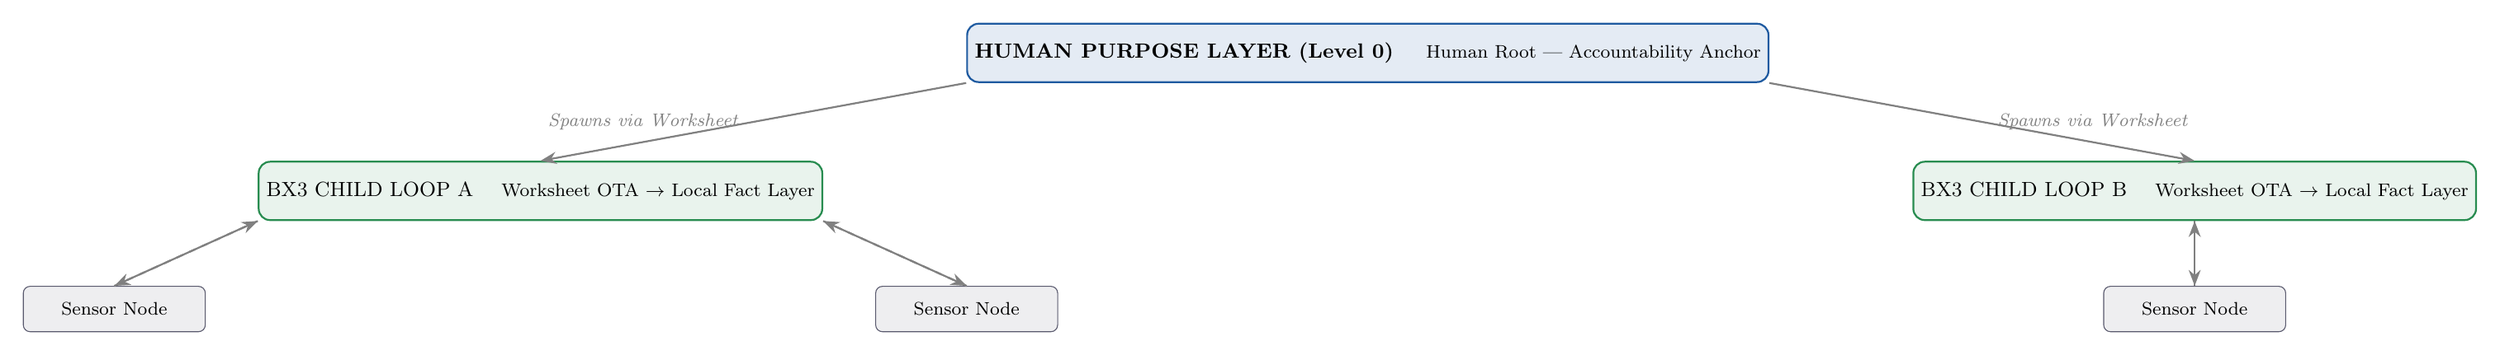
\begin{tikzpicture}[
    root/.style={rectangle, rounded corners=5pt, minimum width=7cm, minimum height=0.9cm,
                 text centered, font=\bfseries\small, draw=humanblue, fill=humanblue!12, thick},
    child/.style={rectangle, rounded corners=5pt, minimum width=4.5cm, minimum height=0.9cm,
                  text centered, font=\small, draw=aigreen, fill=aigreen!10, thick},
    sensor/.style={rectangle, rounded corners=3pt, minimum width=2.8cm, minimum height=0.7cm,
                   text centered, font=\footnotesize, draw=detgray, fill=detgray!10},
    arrow/.style={-{Stealth[length=7pt]}, thick, gray},
    label/.style={font=\footnotesize\itshape, text=gray}
]

\node[root] (root) {HUMAN PURPOSE LAYER (Level 0) \quad \textmd{\footnotesize Human Root --- Accountability Anchor}};

\node[child, below left=1.2cm and 2.2cm of root] (hub1)
    {BX3 CHILD LOOP A \quad \textmd{\footnotesize Worksheet OTA $\to$ Local Fact Layer}};

\node[child, below right=1.2cm and 2.2cm of root] (hub2)
    {BX3 CHILD LOOP B \quad \textmd{\footnotesize Worksheet OTA $\to$ Local Fact Layer}};

\node[sensor, below left=1.0cm and 0.8cm of hub1] (s1) {Sensor Node};
\node[sensor, below right=1.0cm and 0.8cm of hub1] (s2) {Sensor Node};
\node[sensor, below=1.0cm of hub2] (s3) {Sensor Node};

\draw[arrow] (root.south west) -- (hub1.north)
    node[midway, left=3pt, label] {Spawns via Worksheet};
\draw[arrow] (root.south east) -- (hub2.north)
    node[midway, right=3pt, label] {Spawns via Worksheet};
\draw[arrow] (hub1.south west) -- (s1.north);
\draw[arrow] (hub1.south east) -- (s2.north);
\draw[arrow] (hub2.south) -- (s3.north);
\draw[arrow, dashed] (s1.north) -- (hub1.south west)
    node[midway] {};
\draw[arrow, dashed] (s2.north) -- (hub1.south east);
\draw[arrow, dashed] (s3.north) -- (hub2.south);


\end{tikzpicture}
\end{center}
\caption{Recursive spawning and the audit trail. Each spawned node inherits a Worksheet containing the complete system state, ensuring the recursive audit trail cannot be broken by context loss.}
\label{fig:recursive-spawn}
\end{figure}

\vspace{0.8em}

\noindent Every spawned Worksheet maintains a hard-coded pointer to the parent's Purpose, preventing autonomous drift regardless of network conditions or child node failures.

\subsection{Pillar 3: Spatial Firewall}

\textbf{Problem solved:} Soft permissions that can be bypassed, and IP that is protected only by logical access controls rather than physical constraints.

\textbf{Solution:} Access privileges and data resolution tiers are implemented as \textit{physical, hard-coded constraints of the Fact Layer} --- not as software permissions. The system's Fact Layer physically cannot serve data or execute actions beyond a node's provisioned authorization level.

When a Bounds Engine requests a capability beyond its provisioned tier, the Fact Layer does not return a ``Permission Denied'' error. Instead, it triggers an automated resolution pathway --- which may include a commercial upgrade funnel, a human escalation, or a logged denial. Even if a Bounds Engine node is compromised, it cannot access or execute beyond what its Fact Layer gate physically permits. The firewall is in the physics, not the logic.

\subsection{Pillar 4: Root Tunneling}

\textbf{Problem solved:} Abstraction Leakage --- the collapse of organizational hierarchy when a human operator accesses a sub-node, losing global context and breaking the recursive audit trail.

\textbf{Solution:} The \textit{Root-Pipe Protocol} enables the human Purpose Layer to project authority into any node in the system without collapsing the hierarchy. When a tunnel is activated, the node's Purpose is redirected to the human operator's intent, all telemetry and logs are piped to the root dashboard, and all proposed Bounds Engine actions for that node must pass through a \textit{Sandbox Gate} before reaching the Fact Layer.

The Sandbox Gate requires the Bounds Engine to model the projected outcome of any proposed action in a digital twin environment before physical actuators are unlocked \cite{leveson2011}. The human reviews the simulation and provides explicit approval. Only after Human-in-the-Loop validation does the Fact Layer permit physical execution. This provides a high-stakes safety buffer against live-system errors while maintaining the full audit trail.

\subsection{Pillar 5: Bailout Protocol}

\textbf{Problem solved:} The ``Black Box'' problem --- autonomous actions that are orphaned from human responsibility, creating unresolvable legal and operational risk.

\textbf{Solution:} A systemic escalation protocol that guarantees accountability always reaches a human. When any node encounters a state conflict it cannot resolve within its functional bounds, it escalates the exception upward through the recursive system hierarchy, bypassing all machine actors, until it reaches the human Purpose Layer anchor.

\textit{The system fails upward into human consciousness --- never downward into algorithmic chaos.}

No autonomous action is ever orphaned from its human source. Every exception has a traceable escalation path terminating at a named, accountable human.

\textbf{The Forensic Ledger:} Every event in the system is logged simultaneously across three discrete planes --- the Purpose plane (what was authorized), the Bounds Engine plane (what was proposed and why), and the Fact plane (what physical action was taken and what was its outcome). This three-plane ledger provides the forensic standard required for high-stakes regulatory environments, proving that deterministic human oversight was structurally guaranteed throughout the lifecycle of every autonomous event.

% -------------------------------------------------------
\section{The Bounds Engine Used to Build and Improve Fact Layer Systems}
\label{sec:building}

One of the most practically significant implications of the BX3 Framework is that the Bounds Engine's most powerful and appropriate use may not be \textit{operating} within production systems, but \textit{designing and improving} the Fact Layer systems that do. This inversion of the conventional narrative --- the Bounds Engine as a builder of reliability rather than a replacement for it --- is the framework's most actionable contribution for engineers and architects.

\subsection{Pattern Discovery to Rule Encoding}

Bounds Engine systems can be applied to large datasets to discover patterns, correlations, and decision boundaries that would be infeasible for humans to enumerate manually. Once discovered, these patterns can be encoded as deterministic Fact Layer rules, thresholds, or constraint tables --- effectively graduating from probabilistic inference to reliable physical enforcement.

This is the model used in several mature autonomous systems domains, where machine learning is used offline to develop and validate behavioral policies, and only validated, frozen logic is deployed to operational Fact Layer systems. The Bounds Engine's work happens in the design environment; the Fact Layer does the work in the field. The system benefits from the Bounds Engine's pattern recognition capability without inheriting its runtime unpredictability.

\subsection{Bounds Engine-Accelerated Fact Layer Development}

Bounds Engine systems are increasingly used to generate, review, and test deterministic Fact Layer code and constraint specifications. The output of this process is traditional deterministic software --- auditable and certifiable. The Bounds Engine was a tool in the construction process, not a component of the runtime system. This preserves all the reliability properties of deterministic enforcement while dramatically accelerating development.

This pattern resolves a common false trade-off: the assumption that gaining Bounds Engine capability requires accepting Bounds Engine unpredictability at runtime. When the Bounds Engine is used to \textit{build} Fact Layer systems rather than \textit{replace} them, the organization gains speed and generalization at the design phase while retaining reliability and auditability at runtime.

\subsection{Shadow Mode Validation}

A powerful hybrid pattern involves running a Bounds Engine system in parallel with an existing Fact Layer system, comparing proposals against actual enforcement outcomes, and flagging divergences for Purpose Layer review. Over time, Bounds Engine behaviors that consistently improve on the Fact Layer can be promoted --- after explicit Purpose Layer approval --- into the Fact Layer itself.

This pattern is particularly valuable in regulated industries where replacing a certified Fact Layer system requires extensive re-certification. Shadow mode allows Bounds Engine-driven improvements to be identified, validated by the human Purpose Layer, and gradually incorporated without disrupting the certified operational system.

\subsection{The Continuous Improvement Loop}

The BX3 Framework enables a structured continuous improvement cycle that preserves system integrity at every stage:

\begin{enumerate}[noitemsep]
    \item The Fact Layer operates in production, generating performance data and constraint-event logs.
    \item The Bounds Engine analyzes that data, identifying edge cases, inefficiencies, and improvement opportunities.
    \item The Purpose Layer (human anchor) reviews Bounds Engine findings and exercises judgment about which improvements to pursue.
    \item Approved improvements are encoded into the Fact Layer after validation and certification.
    \item The cycle repeats --- the system grows more capable without growing less reliable.
\end{enumerate}

The Purpose Layer remains the gatekeeper through whom all Bounds Engine insight must pass before it becomes Fact Layer logic. Accountability is preserved throughout the improvement process, and the Forensic Ledger records every proposed change and its authorization status.

% -------------------------------------------------------
\section{Application Across Domains}
\label{sec:domains}

The BX3 Framework is not a software engineering principle alone. The same three functional layers --- an accountable Purpose Layer, a bounded Bounds Engine, and a deterministic Fact Layer --- appear across many complex domains. In each case, different types of actors occupy each layer, confirming that the framework's power lies in its functional definitions rather than in any prescription about actor type.

\subsection{Autonomous Systems and Sensor Networks}

In sensor-driven autonomous systems, the BX3 Framework maps directly onto system architecture. Human engineers occupying the Purpose Layer define mission parameters, safety constraints, and acceptable risk envelopes. AI processing layers occupying the Bounds Engine interpret sensor data, handle ambiguous environments, and propose real-time decisions within those constraints. Deterministic control systems occupying the Fact Layer enforce hard constraints --- collision avoidance thresholds, actuator limits, safety interlocks --- that cannot be overridden by the Bounds Engine under any circumstances.

This architecture is critical where the cost of Bounds Engine error is physical and potentially irreversible. The Fact Layer does not need to handle every situation --- only to prevent catastrophic outcomes while the Bounds Engine and Purpose Layer resolve ambiguity.

\subsection{Legal Systems}

Legal systems demonstrate the actor-agnostic property of the BX3 Framework clearly. Legislatures and judges occupy the Purpose Layer --- defining the purpose and interpretation of law, exercising judgment in novel cases, and bearing institutional accountability. AI systems increasingly occupy parts of the Bounds Engine --- assisting with legal research, document analysis, and pattern recognition across case law. The written law itself, procedural rules, and enforcement mechanisms occupy the Fact Layer --- the same statute applies the same way in the same circumstances, regardless of who the parties are.

\subsection{Medicine}

Physicians occupy the Purpose Layer --- exercising judgment incorporating patient context, ethical considerations, and probabilistic reasoning beyond any protocol. AI systems occupy portions of the Bounds Engine --- assisting with imaging analysis, drug interaction checking, and population-level pattern recognition. Drug dosage protocols, surgical checklists, equipment operation specifications, and regulatory requirements occupy the Fact Layer --- deterministic rules that constrain both physician and AI behavior alike.

\subsection{Organizational Design}

Organizations themselves exhibit the BX3 structure. Executive leadership occupies the Intent Layer --- setting strategic direction and bearing accountability. Knowledge workers and AI-augmented teams occupy the Bounds Engine --- interpreting strategy and executing flexibly within organizational guidelines. Policies, compliance requirements, contractual obligations, and financial controls occupy the Fact Layer --- rules that apply consistently regardless of who is executing or what the AI recommends.

\subsection{Biological Cognition}

Notably, the BX3 Framework mirrors the layered architecture of biological cognition \cite{kahneman2011}. The autonomic nervous system and reflexes occupy the Fact Layer --- deterministic, fast, and non-negotiable. Learned heuristics, intuitions, and pattern recognition occupy the Bounds Engine --- efficient responses to familiar situations. Conscious deliberative reasoning occupies the Purpose Layer --- slow, deliberate, and engaged only for genuinely novel, high-stakes, or ethically complex situations.

This convergence suggests the BX3 Framework reflects something deeper than an engineering preference. The same three-layer functional architecture appears to be a near-optimal solution for any system that must simultaneously be reliable, adaptive, and accountable --- regardless of whether that system is biological, organizational, legal, or computational.

% -------------------------------------------------------
\section{Why Deterministic Systems Will Not Be Replaced}
\label{sec:determinism}

A common claim is that sufficiently advanced AI will eventually subsume deterministic software. We argue this position misunderstands the distinct value of determinism as a \textit{property}, not merely a \textit{limitation}.

\subsection{The Value of Determinism is Not Compensable}

Determinism provides properties that probabilistic systems cannot replicate:

\begin{itemize}[noitemsep]
    \item \textbf{Reproducibility:} The ability to reproduce any past output given the same input, enabling debugging, auditing, and legal accountability.
    \item \textbf{Formal verification:} The ability to mathematically prove that a system satisfies certain properties under all possible inputs.
    \item \textbf{Certification:} Regulatory frameworks in aviation, medical devices, financial systems, and safety-critical infrastructure require deterministic behavior as a precondition for approval.
    \item \textbf{Latency:} Hard real-time requirements (microsecond response times) are achievable with deterministic systems and not with current AI inference pipelines.
\end{itemize}

\subsection{The Infrastructure Argument}

Every AI system in production today runs on top of vast deterministic infrastructure: operating systems, databases, networking stacks, authentication systems, billing pipelines, and monitoring tools. The claim that AI will replace software is structurally self-refuting --- the AI systems making this possible are themselves dependent on deterministic software that will not and should not be replaced.

\subsection{The Regulatory and Trust Barrier}

Even in domains where AI could theoretically replace deterministic systems on a performance basis, the practical barriers are substantial. Organizations with core operations dependent on software will not replace functioning, auditable, certified systems with probabilistic alternatives without extraordinary evidence of equivalent reliability and auditability. The burden of proof is appropriately high, and current AI systems do not meet it for most production contexts.

% -------------------------------------------------------
\section{Relationship to Prior Work}
\label{sec:prior}

The BX3 Framework synthesizes established ideas from separation of concerns, sociotechnical systems theory, cybernetics, systems safety, and human-in-the-loop design, but it departs from prior work by defining immutable functional layers according to required properties rather than according to actor type. The closest contemporary analogue is the intelligent sociotechnical systems framework \cite{xu2024}, which similarly emphasizes structured coordination between human and technical components; however, BX3 extends this line of work by explicitly isolating a deterministic Fact Layer and by specifying an actor-agnostic architecture in which any occupant of a layer is bound by that layer's functional obligations.

Recent agentic-AI literature reinforces several needs that BX3 attempts to formalize. Tiered Agentic Oversight (TAO) \cite{kim2025} demonstrates that hierarchical supervision among specialized agents can reduce error propagation in safety-critical settings. BX3 differs in making human accountability the required terminal endpoint of unresolved escalation rather than a high-tier supervisory option. TAO's hierarchy routes to human oversight as a high-risk escalation pathway; BX3 makes this routing unconditional and architectural. Likewise, recent work on production-grade agent architectures \cite{alenezi2026} recommends fail-safe behavior, sandbox-first execution, deterministic fallback workflows, and human approval gates for risky actions; BX3 incorporates these concerns as named architectural pillars --- most notably the Sandbox Gate and Bailout Protocol --- rather than as implementation heuristics.

While recent agentic-architecture literature recommends sandbox-first execution and human approval gates for high-risk actions, BX3 specifies a narrower architectural requirement: proposed interventions must be evaluated in a digital twin and cleared through a role-bounded Sandbox Gate tied to Root Tunneling authority before the Fact Layer is unlocked.

BX3 also sits naturally alongside emerging governance and compliance literature. Koch \cite{koch2026} argues that standards such as ISO/IEC 42001 \cite{iso2023} and the NIST AI RMF \cite{nist2023} do not themselves provide implementable runtime guardrails, and instead require translation across governance, design-time, runtime, and assurance layers. BX3 may be read as one candidate architecture for that translation. In parallel, formal-verification approaches such as the Lean-Agent Protocol \cite{rashie2026} show how proposed agentic actions can be forced through deterministic verification gates before execution. BX3 generalizes that intuition beyond theorem proving: wherever execution must remain non-probabilistic, a protected deterministic layer is architecturally indispensable.

The recurrence of layered models in global AI governance discourse \cite{sabah2026} further suggests that complex AI systems are increasingly being understood through stratified functional abstractions, although those models are policy-descriptive rather than engineering-prescriptive.

\section{Conclusion}
\label{sec:conclusion}

The question of how humans, AI, and traditional software should relate to one another is not merely a technical question. It is an architectural, organizational, ethical, and regulatory question with significant and growing practical consequences.

The BX3 Framework proposes a principled and universal answer. It organizes any complex system into three functional layers --- Purpose, Bounds Engine, and Fact --- each defined by the properties it must maintain rather than by the type of actor that occupies it. Any actor capable of satisfying a layer's functional requirements may occupy that layer: human, AI, mechanical, institutional, or hybrid. What cannot vary are the properties themselves --- accountability in the Purpose Layer, boundedness in the Bounds Engine, and determinism in the Fact Layer.

This actor-agnostic definition is the framework's most important contribution beyond its predecessors. It makes the BX3 Framework applicable to the full range of systems that exist and the full range of systems that are coming: human-only organizations, fully automated pipelines, multi-agent AI architectures, and hybrid compositions that do not yet have names. In each case, the framework asks the same three questions: Is there an accountable layer that sets purpose and bears responsibility? Is there a bounded layer that reasons and proposes within defined constraints? Is there a deterministic layer that enforces, validates, and audits? If any layer is missing or its properties are not maintained, the system is architecturally incomplete --- regardless of how capable its components are individually.

The BX3 Framework is not entirely new. Its pattern is visible in legal systems, medical practice, autonomous vehicles, biological cognition, and organizational design --- wherever reliable systems have been built to handle a world that is simultaneously rule-bound and unpredictable. What is new is the urgency of making the pattern explicit, naming its layers by function rather than actor, and building from it deliberately --- at a moment when the temptation to collapse these roles, and the cost of doing so, have never been higher.

% -------------------------------------------------------
\section*{Acknowledgments}

The author wishes to acknowledge the foundational contributions of the researchers cited herein, whose work across control theory, sociotechnical systems, and computer science provides the shoulders on which this synthesis stands.

% -------------------------------------------------------
\bibliographystyle{plainnat}
\bibliography{bx3framework}

\vspace{2em}
\hrule
\vspace{0.5em}
\noindent\small\textit{This work has not undergone peer review. Comments and correspondence are welcomed.}

\end{document}
